\section{基础知识}
\begin{enumerate}
    \item 考虑下列定义于资产$X$上的效用函数为风险厌恶型投资者的效用函数。
    \begin{enumerate}[label=(\arabic*)]
        \item $U(X)=\ln(X)$
        \item $\displaystyle U(X)=-\frac{1}{X}$
    \end{enumerate}
    \pro
    \begin{enumerate}[label=(\arabic*)]
        \item $\displaystyle U'(X)=\frac{1}{X} \geqslant 0, U''(X)=-\frac{1}{X^2} \leqslant 0, \forall X>0,$不等号恒成立,故这是风险厌恶型投资者的效用函数。
        \item $\displaystyle U'(X)=\frac{1}{X^2} \geqslant 0, U''(X)=-\frac{2}{X^3} \leqslant 0, \forall X \neq 0,$不等号恒成立,故这是风险厌恶型投资者的效用函数。
    \end{enumerate}
    \item 若下列效用函数为风险厌恶型投资者的效用函数,求$a$的取值范围。
    \begin{enumerate}[label=(\arabic*)]
        \item $U(X)=-X^{-a}$
        \item $U(X)=-\mathrm{e}^{-aX}$
        \item $\displaystyle U(X)=\frac{X^a}{a}$
    \end{enumerate}
    \sol
    \begin{enumerate}[label=(\arabic*)]
        \item $\displaystyle U'(X)=\frac{a}{X^{a+1}} \geqslant 0, U''(X)=-\frac{a(a+1)}{X^{a+2}} \leqslant 0 \Rightarrow a \geqslant 0$,而$a=0$时,$U(X)=-1,U'(X)=0,U'(X)=0$不满足至少存在一点使得不等号成立,故$a > 0$.
        \item $\displaystyle U'(X)=a\mathrm{e}^{-aX} \geqslant 0, U''(X)=-a^2\mathrm{e}^{-aX} \leqslant 0 \Rightarrow a \geqslant 0$,而$a=0$时,$U(X)=-1,U'(X)=0,U'(X)=0$不满足至少存在一点使得不等号成立,故$a > 0$.
        \item $\displaystyle U'(X)=X^{a-1} \geqslant 0, U''(X)=(a-1)X^{a-2} \leqslant 0 \Rightarrow a \leqslant 1$,而$a=1$时,$U(X)=X,U'(X)=1,U'(X)=0$不满足至少存在一点使得不等号成立,故$a < 1$.
    \end{enumerate}
    \item 考虑以下两种投资A和B:
    \begin{center}
        \setlength{\tabcolsep}{17mm}{
        \begin{tabular}{c|c|c|c}
            \hline
            \multicolumn{2}{c|}{A} & \multicolumn{2}{|c}{B} \\ \hline
            收益 & 概率 & 收益 & 概率 \\ \hline
            2 & 0.2 & 3 & 0.6 \\ \hline
            3 & 0.3 & 6 & 0.4 \\ \hline
            5 & 0.5 & & \\ \hline
        \end{tabular}}
    \end{center}
    分别利用三个随机优势准则分析哪种投资更优,并说明原因。\\
    \sol
    \begin{enumerate}[label=(\arabic*)]
        \item FSD准则:写出两者的分布函数:
        \[F_A(r)=\begin{cases}
            0, & r < 2\\
            0.2, & 2 \leqslant r < 3\\
            0.5, & 3 \leqslant r < 5\\
            1, & r \geqslant 5
        \end{cases},F_B(r)=\begin{cases}
            0, & r < 3\\
            0.6, & 3 \leqslant r < 6\\
            1, & r \geqslant 6
        \end{cases}\]
        当$2 \leqslant r<3$和$5 \leqslant r < 6$时,B更优,当$3 \leqslant r \leqslant 5$时,A更优。
        \item SSD准则:写出两者分布函数的分布函数:
        \[F_{FA}(r)=\begin{cases}
            0, & r < 2\\
            0.2, & 2 \leqslant r < 3\\
            0.7, & 3 \leqslant r < 5\\
            1.7, & r \geqslant 5
        \end{cases},F_{FB}(r)=\begin{cases}
            0, & r < 3\\
            0.6, & 3 \leqslant r < 6\\
            1.6, & r \geqslant 6
        \end{cases}\]
        B更优。
        \item TSD准则:写出两者分布函数的分布函数的分布函数:
        \[F_{FFA}(r)=\begin{cases}
            0, & r < 2\\
            0.2, & 2 \leqslant r < 3\\
            0.9, & 3 \leqslant r < 5\\
            2.6, & r \geqslant 5
        \end{cases},F_{FFB}(r)=\begin{cases}
            0, & r < 3\\
            0.6, & 3 \leqslant r < 6\\
            2.2, & r \geqslant 6
        \end{cases}\]
        而$\mu_A=3.8 \leqslant \mu_B=4.2$,则无法判断A、B的优劣。
    \end{enumerate}
    \item 假设一个投资方案A的分布函数由以下函数给出,描述FSD准则。
    \[F_A(x)=\begin{cases}
        0, & 0 \leqslant x < 1\\
        0.1, & 1 \leqslant x < 2\\
        0.8, & 2 \leqslant x < 4\\
        1, & x \geqslant 4
    \end{cases}\]
    假设另外三个投资方案B、C和D的收益分布函数由以下函数给出,分析投资机会A优于以下哪个投资方案?
    \[F_B(x)=\begin{cases}
        0, & 0 \leqslant x < 1\\
        0.2, & 1 \leqslant x < 2\\
        0.7, & 2 \leqslant x < 4\\
        1, & x \geqslant 4
    \end{cases} \quad F_C(x)=\begin{cases}
        0, & 0 \leqslant x < 1\\
        0.1, & 1 \leqslant x < 2\\
        0.6, & 2 \leqslant x < 4\\
        1, & x \geqslant 4
    \end{cases} \quad F_D(x)=\begin{cases}
        0, & 0 \leqslant x < 1\\
        0.1, & 1 \leqslant x < 3\\
        0.6, & 3 \leqslant x < 4\\
        1, & x \geqslant 4
    \end{cases}\]
    \sol\\
    描述FSD准则:对于投资机会A与其他任意投资机会Z,A优于Z的充要条件是$\forall x \in R$,$F_A(x) \leqslant F_Z(x)$(不等号至少在一点上成立)。\\
    当$1 \leqslant x < 2$时,A优于B。
    \item 假设三个投资方案A、B和C的收益分布函数均服从正态分布,其期望和标准差由以下表格给出:
    \begin{center}
        \setlength{\tabcolsep}{20mm}{
        \begin{tabular}{c|c|c}
            \hline
            投资方案 & 期望($\mu$) & 标准差($\sigma$) \\ \hline
            A & 12\% & 4\% \\ \hline
            B & 10\% & 3\% \\ \hline
            C & 5\% & 1\% \\ \hline
        \end{tabular}}
    \end{center}
    利用SSD准则判断这三个投资机会之间的优劣,并说明原因。\\
    \sol\\
    利用标准正态函数计算分布函数,$\forall x,$
    \[\begin{array}{ll}
        & \displaystyle F_{FA}(x) = \int_{-\infty}^x \frac{1}{0.04\sqrt{2\pi}}\exp\left[-\frac{(x-0.12)^2}{0.0032}\right] \, \mathrm{d}x = \Phi \left(\frac{x-0.12}{0.04}\right),\\
        & \displaystyle F_{FB}(x) = \int_{-\infty}^x \frac{1}{0.03\sqrt{2\pi}}\exp\left[-\frac{(x-0.1)^2}{0.0018}\right] \, \mathrm{d}x = \Phi \left(\frac{x-0.1}{0.03}\right),\\
        & \displaystyle F_{FC}(x) = \int_{-\infty}^x \frac{1}{0.02\sqrt{2\pi}}\exp\left[-\frac{(x-0.05)^2}{0.0002}\right] \, \mathrm{d}x = \Phi \left(\frac{x-0.05}{0.01}\right).
    \end{array}\]
    可以大致画出曲线:
    \begin{center}
        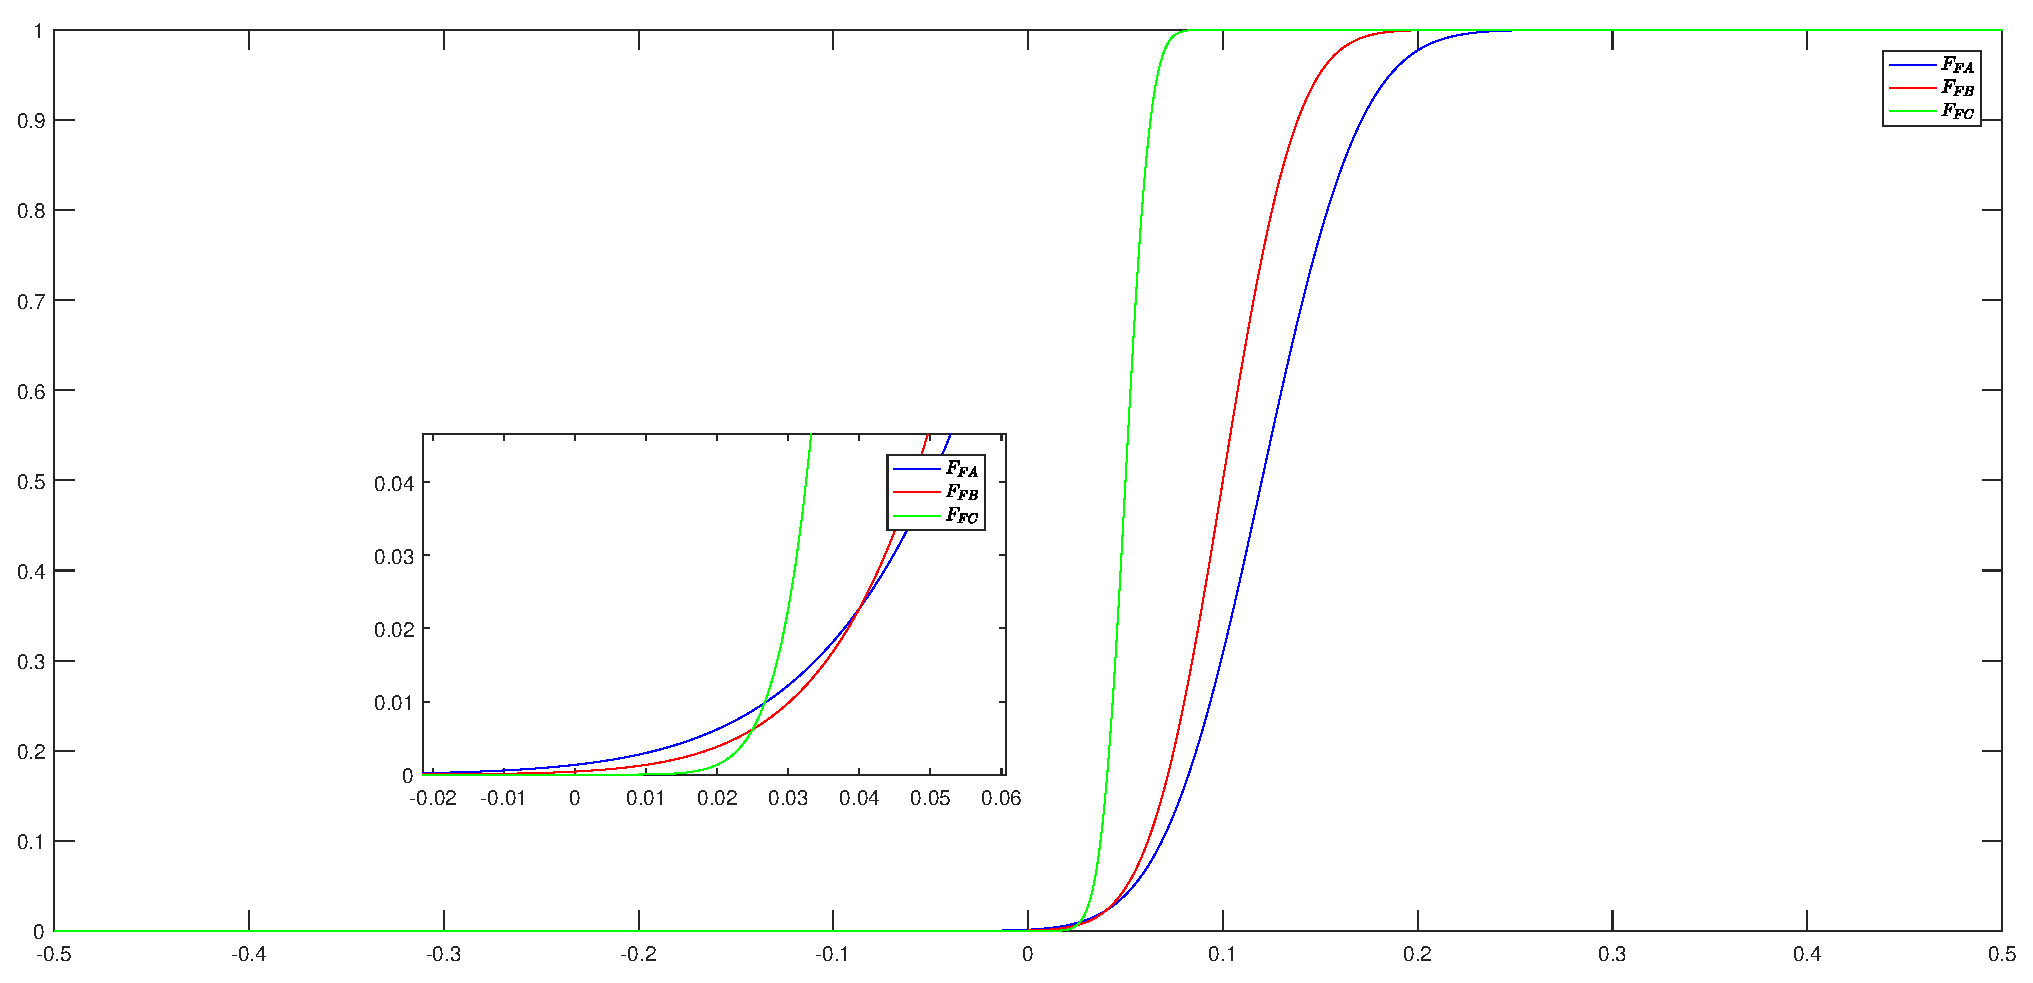
\includegraphics[scale=0.49]{1_5.eps}
    \end{center}
    则当$x < 0.025$时,C更优,当$0.025 < x < 0.04$时,B更优,当$x > 0.04$时,A更优。\\
    Matlab绘图命令如下:
\begin{lstlisting}
x = -0.5:0.001:0.5;
ffa = normcdf(x, 0.12, 0.04);
ffb = normcdf(x, 0.1, 0.03);
ffc = normcdf(x, 0.05, 0.01);
plot(x, ffa, 'b');
hold on;
plot(x, ffb, 'r');
plot(x, ffc, 'g');
\end{lstlisting}
% l = legend('$F_{FA}$', '$F_{FB}$', '$F_{FC}$');
% set(l, 'Interpreter', 'latex');
\end{enumerate}
\clearpage